%%%  _____               _
%%% |_   _|__  ___  _ __(_) __ _
%%%   | |/ _ \/ _ \| '__| |/ _` |
%%%   | |  __/ (_) | |  | | (_| |
%%%   |_|\___|\___/|_|  |_|\__,_|
%%%
%%% TCC de Bianca Miyabe Santos Freitas
%%% Licenciatura em Física - UFSCar, Sorocaba
%%%

\chapter{Fundamentação Teórica}

Conforme descrito no Capítulo de Introdução, para o estudo da Computação Quântica e da Informação Quântica, são necessários alguns recursos provenientes da Mecânica Quântica bem como a construção de análogos quânticos para o processamento dessa informação. As seções a seguir apresentarão a fundamentação teórica e os recursos matemáticos necessários para o desenvolvimento da simulação proposta na Metodologia.

\section{Conceitos básicos de Álgebra Linear}
A Álgebra Linear é o estudo dos vetores que descrevem o espaço e consequentemente das operações nesses espaços vetoriais. Para o desenvolvimento desse trabalho, serão necessários reconhecer as notações descritas na Tabela~\ref{tab:notação}.

\begin{table}[ht!]
  \centering
  \caption{Notações utilizadas nas operações de Mecânica Quântica e sua respectiva descrição. O estilo das notações é conhecido como Notação de Dirac para Álgebra Linear.}\label{tab:notação}
  \begin{tabular}{cc}
    \toprule
    {\textbf{Notação}} & {\textbf{Descrição}}\\
    \midrule
    $\ket{\psi}$   & Vetor conhecido como \textit{ket} \\
    $\bra{\psi}$   & Vetor dual de um \textit{ket} conhecido como \textit{bra} \\
    $\braket{\psi|\varphi}$   & Produto interno entre os vetores $\ket{\psi}$ e $\ket{\varphi}$ \\
    $\ket{\psi} \otimes \ket{\varphi}$   & Produto tensorial entre os vetores $\ket{\psi}$ e $\ket{\varphi}$ \\
    $\ket{\psi}\ket{\varphi}$     & Abreviação do produto tensorial entre $\ket{\psi}$ e $\ket{\varphi}$ \\
    $A^*$     &  Conjugado complexo da Matriz A \\
    \bottomrule
  \end{tabular}
  \fonte{Adaptada de \textcite{chuang}.}
\end{table}

A descrição da Mecânica Quântica é feita considerando como base o espaço vetorial chamado \textit{Espaço de Hilbert} $\mathcal{H}$, sendo este um espaço complexo, vetorial e linear. Um \textit{ket} é um vetor arbitrário de $\mathcal{H}$, sua representação é descrita por:

\begin{equation}\label{eq:ketpsi}
\ket{\psi} = [\psi_1,...,\psi_n]^T
\end{equation}

Todo \textit{ket} possui um vetor dual, ou conjugado complexo que também pertence à $\mathcal{H}$, chamado de \textit{bra}, de modo que:

\begin{equation}\label{eq:brapsi}
\bra{\psi} = [\psi_1^*,...,\psi_n^*]
\end{equation}

O produto tensorial entre dois \textit{kets} é definido por:

\begin{equation}\label{eq:tensorket}
\ket{\psi} \otimes \ket{\varphi} = \ket{\psi}\ket{\varphi} =\ket{\psi \varphi} =\left[\begin{array}{c}\psi_1 \varphi_1 \\ \psi_1 \varphi_2 \\ \vdots \\ \psi_1 \varphi_n \\ \psi_2 \varphi_1 \\ \psi_2 \varphi_2 \\ \vdots \\ \psi_2 \varphi_n \\ \vdots \\ \psi_m \varphi_2 \\ \psi_m \varphi_2 \\ \vdots \\ \psi_m \varphi_n\end{array}\right]
\end{equation}

Podemos também realizar o produto tensorial de duas matrizes, de modo que:

\begin{equation}\label{eq:tensormatrix}
A \otimes B=\left[\begin{array}{cccc}
A_{11} B & A_{12} B & \cdots & A_{1 n} B \\
A_{21} B & A_{22} B & \cdots & A_{2 n} B \\
\vdots & \vdots & \ddots & \vdots \\
A_{m 1} B & A_{m 2} B & \cdots & A_{m n} B
\end{array}\right]_{m p \times n q}
\end{equation}

O conjugado complexo de uma Matrix é definido pela Matriz transposta dos seus elementos, de modo que:

\begin{equation}\label{eq:conjugadomatrix}
A^T = \left[\begin{matrix}
a & b \\
c & d
\end{matrix}\right]^T = \left[\begin{matrix}
a & c \\
b & d
\end{matrix}\right]
\end{equation}

Os recursos apresentados acima, serão utilizados durante o trabalho e principalmente na descrição da seção~\ref{Mecanicaquantica}.

\section{Mecânica Quântica}\label{Mecanicaquantica}



\section{Qubits}

As definições de qubits descritas nesse tópico baseiam-se principalmente nas ideias apresentadas por \textcite{chuang} e \textcite{CompInfoQuantica}.

Qubits são elementos fundamentais da computação quântica. Eles são usados para representar informações binárias (zeros e uns) e são capazes de armazenar e processar muito mais informações que os bits convencionais usados na computação clássica. Isso é possível graças ao fato de que, enquanto os bits tradicionais podem estar em dois estados (ligado ou desligado), os qubits podem estar em um estado de superposição, o que permite que eles representem simultaneamente vários estados ou informações diferentes. Isso significa que os qubits podem armazenar muito mais informação em um espaço muito menor conforme salientado na~\ref{tabelabit}.

Podemos começar a descrição de um qubit como uma superposição dos estados quânticos $\ket{0}$ e $\ket{1}$, de modo a representá-los pela combinação linear dada por
\begin{equation}\label{eq:psi}
\ket{\psi} = \alpha \ket{0} + \beta \ket{1},
\end{equation}
com $\alpha$ e $\beta$ parametrizados por \(\alpha^{2} + \beta^{2} = 1\).

Os números $\alpha$ e $\beta$ são complexos e determinam as amplitudes probabilísticas da obtenção dos estados quânticos. O estado descrito por $\ket{\psi}$ é uma superposição dos estados quânticos $\ket{0}$ e $\ket{1}$, ou seja, seguindo os postulados da mecânica quântica, o qubit pode existir num estado contínuo entre $\ket{0}$ e $\ket{1}$ porém, ao ser medido, colapsando o sistema, retornará apenas os valores de $\ket{0}$ ou $\ket{1}$ com as probabilidades $\alpha$ e $\beta$ associadas.

Um recurso para visualizar o comportamento de qubits é sua representação geométrica chamada de Esfera de Boch. Como entidades quânticas não são observáveis diretamente e frequentemente são expressas por recursos matemáticos, a visualização da superposição dos estados de um qubit utilizando a Esfera de Boch facilita, ainda que ligeiramente, sua compreensão.

Em primeiro lugar, vale lembrar que o qubit, descrito por $\ket{\psi}$, está parametrizado e podemos reescrever~\eqref{eq:psi} em coordenadas polares
\begin{equation}
\ket{\psi}=e^{i \gamma}\Biggl(\cos \frac{\theta}{2}\ket{0}+e^{i \varphi} \sen \frac{\theta}{2}\ket{1}\Biggr).
\end{equation}
O termo \(e^{i\gamma}\) não possui efeitos observáveis na representação geométrica e portanto, podemos simplificar a equação acima, obtendo
\begin{equation}\label{eq:coordpolarpsi}
\ket{\psi}=\Biggl(\cos \frac{\theta}{2}\ket{0}+e^{i \varphi} \sen \frac{\theta}{2}\ket{1}\Biggr),
\end{equation}
com $\theta$ e $\varphi$ sendo números reais correspondentes aos ângulos entre os eixos $z, y$ e $y, x$ respectivamente, conforme a
Figura~\ref{fig:bloch}.

\begin{figure}[ht!]
\centering
\caption{Representação gráfica de um qubit como um ponto sob a superfície da Esfera de Bloch.}\label{fig:bloch}
% Adaptado de https://tex.stackexchange.com/questions/345420/how-to-draw-a-bloch-sphere
\begin{blochsphere}[radius=3cm,rotation=-110,opacity=0]
  \drawLongitudeCircle[]{-110};
  \drawLatitudeCircle[style={dashed}]{0};
  \labelLatLon{ket0}{90}{0};
  \labelLatLon{ket1}{-90}{0};
  \labelLatLon{ketminus}{0}{180};
  \labelLatLon{ketplus}{00}{0};
  \labelLatLon{ketpluspi2}{0}{-90};  % Longitude seems to be defined in the "wrong" direction, hence the minus
  \labelLatLon{ketplus3pi2}{0}{-270};
  \labelLatLon{psi}{45}{-45};

  \draw[-latex] (0,0) -- (ket0) node[pontinho=blue] {} node[below right,inner sep=.5mm] at (ket0) {$z$} node[above,inner sep=.5mm] at (ket0) {$\ket{0}$};
  \draw[-latex,dashed,opacity=0.2] (0,0) -- (ket1);
  \node[pontinho=blue] at (ket1) {} node[below,inner sep=.5mm] at (ket1) {$\ket{1}$};
  \draw[-latex] (0,0) -- (ketplus) node[below,inner sep=.5mm] at (ketplus) {$x$};
  \draw[-latex] (0,0) -- (ketpluspi2) node[below,inner sep=.5mm] at (ketpluspi2) {$y$};
  \draw[-latex] (0,0) -- (psi) node[pontinho=blue] {} node[above] {$\ket{\psi}$};

  \coordinate (origin) at (0,0);
  {
    \setDrawingPlane{0}{0}
    \draw[current plane,dashed] (0,0) -- (-90+45:{cos(45)*3cm}) coordinate (psiProjectedEquat) -- (psi);
    \pic[current plane,draw,fill=orange!20,fill opacity=.5,text opacity=1,pic text=$\varphi$,angle eccentricity=2.2,left]{angle=ketplus--origin--psiProjectedEquat};
  }
  { \setLongitudinalDrawingPlane{45}
    \pic[current plane,draw,fill=orange!20,fill opacity=.5,text opacity=1,pic text=$\theta$,angle eccentricity=1.5]{angle=psi--origin--ket0};
  }
\end{blochsphere}
% 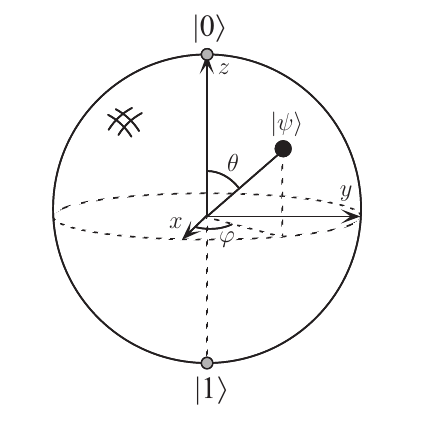
\includegraphics[width=0.5\linewidth]{boch.png}
\fonte{Adaptado de \textcite{chuang}.}
\end{figure}

%EXPLICAR COMO FUNCIONA O ARMAZENAMENTO DE INFORMAÇÃO NO QUBIT E COMO FUNCIONA A MEDIDA DE UM ESTADO

\section{Operadores Quânticos}

Na Mecânica Quântica, um Operador Quântico é um objeto matemático que representa uma propriedade física observável de um sistema quântico sendo fundamentais para a teoria quântica porque fornecem uma maneira de descrever e prever os resultados de medidas em sistemas quânticos. Eles são representados por matrizes ou operadores lineares em um espaço de Hilbert, que é o espaço de estados possíveis do sistema sendo utilizados principalmente em operações lógicas realizadas em um sistema de qubits. As portas quânticas, que são equivalentes às portas lógicas na computação clássica, são implementadas como operadores quânticos que atuam em um ou mais qubits. As próximas subseções serão utilizadas para explicar os principais operadores/portas lógicas quânticas e como eles atuam em um qubit \cite{jorcuvich}.

\subsection{Matrizes de Pauli}\label{sec:pauli}

Segundo \textcite{chuang}, matrizes de Pauli são um conjunto de três matrizes hermitianas e unitárias amplamente utilizadas na computação quântica. As matrizes são denotadas por $\sigma_x$, $\sigma_y$ e $\sigma_z$, e são definidas por:

\begin{equation}
\sigma_x=\left(\begin{array}{cc}
0 & 1 \\
1 & 0
\end{array}\right), \quad \sigma_y=\left(\begin{array}{cc}
0 & -i \\
i & 0
\end{array}\right), \quad \sigma_z=\left(\begin{array}{cc}
1 & 0 \\
0 & -1
\end{array}\right)
\end{equation}

A matriz $\sigma_x$ é também conhecida como a matriz de Pauli X, enquanto $\sigma_y$ é a matriz de Pauli Y, e $\sigma_z$ é a matriz de Pauli Z. As matrizes de Pauli são importantes porque elas formam a base do espaço de Hilbert de um único qubit, e podem ser usadas para construir operadores mais complexos que atuam em vários qubits.

\subsection{Porta Lógica Controlled-NOT Quântica}\label{sec:cnot}
As matrizes de Pauli são frequentemente usadas na construção de portas lógicas quânticas. Por exemplo, a porta NOT quântica, que é usada para inverter o estado de um qubit, é construída a partir da matriz de Pauli X. A porta Controlled-NOT Quântica, ou \(\CNOT\), que é usada para realizar operações lógicas em dois qubits, também é construída a partir de matrizes de Pauli \cite{CompInfoQuantica}. 
A porta \(\CNOT\) opera de tal forma que o estado de um qubit de controle determina a operação realizada em outro qubit alvo. A matriz que representa a porta \(\CNOT\) é dada por:

\begin{equation}
\CNOT = \begin{pmatrix}
1 & 0 & 0 & 0 \\
0 & 1 & 0 & 0 \\
0 & 0 & 0 & 1 \\
0 & 1 & 1 & 0
\end{pmatrix} 
\end{equation}

A Porta Lógica \(\CNOT\) é usada para implementar operações condicionais e permutações entre qubits. Ela é usada para criar circuitos lógicos quânticos mais complexos sendo é uma versão geral da porta CNOT clássica, pois ela pode ser aplicada a todos os qubits, não apenas dois. Na porta \(\CNOT\), o qubit de controle é usado para controlar o estado de outro qubit (alvo). Se o qubit de controle estiver em 1, o estado do qubit alvo será invertido, mas se o qubit de controle estiver em 0, o estado do qubit alvo não será alterado. A porta \(\CNOT\) também pode ser usada para realizar permutações, ou seja, trocar o estado de dois qubits.
Note que a matriz da porta \(\CNOT\) é uma matriz $4 \times 4$ que pode ser escrita como uma combinação linear das matrizes de Pauli X, Y e Z, bem como da matriz de identidade. Esta é uma propriedade geral das portas lógicas quânticas: elas podem ser construídas a partir de matrizes que são combinações lineares das matrizes de Pauli e da matriz de identidade \cite{chuang}.

\subsection{Porta Lógica Hadamard Quântica}\label{sec:had}

A Porta Lógica Hadamard Quântica \(\HAD\) é uma porta lógica quântica que transforma o estado de um qubit em seu estado oposto com 50\% de probabilidade. Ela pode ser usada para realizar operações de entrelaçamento entre qubits, o que permite a implementação de algoritmos quânticos complexos. A porta \(\HAD\) foi desenvolvida com o objetivo de permitir o controle preciso de qubits em circuitos quânticos \cite{jorcuvich}. Ela é representada por um matrix unitário de 2x2, que é definido como:

\begin{equation}
\HAD= \frac{1}{\sqrt{2}} \begin{pmatrix*}[r]
1 & 1 \\
1 & -1
\end{pmatrix*}
\end{equation}


\section{Emaranhamento Quântico}

%O emaranhamento quântico é o fenômeno pelo qual partículas elementares, como fótons, elétrons e outras, ligam-se entre si de tal maneira que um objeto passa a ter quase que uma única identidade. Neste estado, um objeto passa a ter propriedades que estão além dos limites da mecânica quântica. Em outras palavras, o emaranhamento quântico é um estado no qual duas partículas interagem de forma tal que elas compartilham o mesmo estado e não podem ser descritas independentemente. Por exemplo, dois fótons entrelaçados podem ser entendidos como uma única partícula, mesmo que eles estejam distantes um do outro. O emaranhamento quântico pode ser usado para criar ligações entre partículas e objetos distantes, o que abre portas para o desenvolvimento de novas tecnologias, como a computação quântica.
%
%Etapas do Emaranhamento Quântico de Qubits
%
%\begin{itemize}
%\item 1. Preparação:  O primeiro passo é preparar os qubits individuais. Isso pode ser feito carregando os qubits em computadores quânticos ou usando dispositivos quânticos especializados, como lasers.
%
%\item 2. Entrelaçamento: Em seguida, os qubits são entrelaçados, o que significa que eles são interconectados de modo que as informações entre eles sejam compartilhadas. Isso pode ser feito usando técnicas como a interferência quântica.
%
%\item 3. Operações: Uma vez que os qubits estão entrelaçados, as operações quânticas podem ser realizadas neles. As operações podem incluir a realização de computações quânticas complexas, o armazenamento de informações quânticas ou o envio de informações entre qubits.
%
%\item 4.Saída: Por fim, os qubits podem ser desentrelaçados para obter a saída desejada. Isso pode ser feito usando técnicas como a interferência quântica inversa. A saída pode incluir informações codificadas nos qubits, como um resultado de uma computação quântica.
%
%\end{itemize}



\section{Teletransporte Quântico}
%O  Teletransporte Quântico
%
%O Teletransporte Quântico é um processo de transferência de informação quântica entre dois pontos, usando mecanismos quânticos. Essa transferência pode ocorrer quase instantaneamente, independentemente da distância entre os dois pontos.
%O Teletransporte Quântico é baseado em princípios da mecânica quântica, que descrevem como os estados quânticos podem ser compartilhados entre partículas e aplicados aos sistemas de informação. O Teletransporte Quântico foi descoberto pela primeira vez pela física austríaca Anton Zeilinger, em 1998. Ela escobriu que, usando um fenômeno conhecido como entrelaçamento quântico, é possível transferir informação instantaneamente entre dois pontos. O princípio básico do teletransporte quântico é que dois partículas, como elétrons, átomos ou fótons, podem ser entrelaçados, ou ligados entre si. Quando isso acontece, qualquer mudança na configuração de uma partícula será imediatamente refletida na outra, mesmo que elas estejam separadas por uma distância enorme. Isso significa que informação pode ser enviada instantaneamente entre dois pontos distantes.
%
%Embora o teletransporte quântico ainda esteja em fase experimental, já foi usado para transferir informações básicas como posição, polarização e estado de spin entre dois pontos separados. A tecnologia ainda precisa desenvolver muito antes de poder ser usada para transferir informações mais complexas, como imagens ou dados.
%
%Na prática, o Teletransporte Quântico permite que um estado quântico seja transferido de um lugar para outro, sem que nenhuma informação seja transferida entre os locais. Isso significa que um estado quântico pode ser transmitido de uma parte do universo para outra sem que nenhuma informação seja trocada entre eles.
%O Teletransporte Quântico é usado em diversas áreas científicas, como criptografia, computação quântica, comunicação segura e muito mais. Também pode ser usado para transferir informações confidenciais de um lugar para outro, impedindo que terceiros interceptem a informação.


\section{Protocolo de Teletransporte Quântico}

A descrição deste protocolo foi baseada em \textcite{chuang, jorcuvich, CompInfoQuantica, benschu}. A realização de um protocolo de Teletransporte Quântico consiste, essencialmente, em uma série de operações que possuem por objetivo principal fazer com que uma mensagem, ou na linguagem quântica, um estado quântico, se teletransporte entre dois pontos distintos fisicamente.
Como em qualquer outra operação computacional é necessária a existencia de um circuito lógico, nesse caso, quântico que media as operações. Esse circuito consistirá nas combinações das portas lógicas \(\CNOT\), Haddamard, portas de medição e as portas \(\XXX\) e \(\ZZZ\) conforme a Figura~\ref{fig:protocoloteletransporte}

\begin{figure}[ht!]
\centering
\caption{Protocolo de Teletransporte Quântico mediado pelo circuito com as portas \(\CNOT\), Hadamard, Medição aplicadas no Local \(A\) e as portas \(\XXX\) e \(\ZZZ\) aplicadas no Local \(B\).}\label{fig:protocoloteletransporte}
\begin{quantikz}[slice style=blue]
\lstick{$\ket{\psi}$} & \qw & \qw & \qw \slice{$\ket{\psi_0}$} & \ctrl{1} \slice{$\ket{\psi_1}$} & \gate{H} \slice{$\ket{\psi_2}$} & \meter{$M_1$} & \cw  & \cw & \cwbend{2}\\
\lstick{$\ket{q_x}$} & \gate{H}\gategroup[2,steps=2,style={dashed,rounded corners,fill=blue!20, inner xsep=2pt}, background,label style={label position=below,anchor=north,yshift=-0.2cm}]{{Emaranhamento}} & \ctrl{1} & \midstick[2]{$\ket{\beta_{00}}$} \qw & \targ{} & \qw & \meter{$M_2$} & \cwbend{1} \\
\lstick{$\ket{q_y}$} & \qw & \targ{} \arrow{r} &  & \qw & \qw & \qw & \gate{X} & \qw & \gate{Z} &  \qw\rstick{$\ket{\psi}$}
\end{quantikz}
\fonte{Adaptado de }
\end{figure}

No inicio do protocolo é necessário que tenhamos um par de qubits emaranhados nas bases de Bell, no estado $\ket{\beta_{00}}$, que podemos representar pela expressão
\begin{equation}\label{eq:bell00}
 \ket{\beta_{00}} = \frac{\ket{00} + \ket{11}}{\sqrt{2}}.
\end{equation}

Um dos qubits do par emaranhado em~\eqref{eq:bell00} é mantido em \(A\) e o outro necessariamente precisa estar em \(B\) para que exista um canal de comunicação entre essas partes. Além do par emaranhado, em \(A\) teremos o estado quântico a ser enviado, ou seja sua mensagem dada por $\ket{\psi}$, segundo a Equação~\eqref{eq:psi}.
% \begin{equation}\label{psi}
%  \ket{\psi} = \alpha \ket{0} + \beta \ket{1}.
% \end{equation}
De posse do par emaranhado e da mensagem, o protocolo é iniciado com a aplicação da porta \(\CNOT\) entre $\ket{\psi}\ket{\beta_{00}}$, que chamaremos de $\ket{\psi_0}$. A porta \(\CNOT\) possui como alvo o qubit $\ket{q_y}$ e como qubit de controle $\ket{q_x}$. Isso indica que a porta \(\CNOT\) irá modificar $\ket{q_y}$ de acordo com o estado de $\ket{q_x}$ de modo que:


\begin{theo}{Operação \(\CNOT\)}{cnot}
  A operação \(\CNOT\):
  \begin{enumerate}[label=\roman*.,left=0pt]
    \item Inverte o qubit alvo, caso o qubit de controle esteja no estado $\ket{1}$;
    \item Não realizar nenhuma operação no qubit alvo, caso o controle esteja no estado $\ket{0}$.
  \end{enumerate}
\end{theo}

Dessa maneira, aplicando a definição~\ref{def:cnot} no estado dado por $\ket{\psi_0}$
\begin{align}\label{eq:cnotpsi0}
  \CNOT \ket{\psi_0} &= \CNOT \ket{\psi} \ket{\beta_{00}} \nonumber \\
                     &= \CNOT \frac{1}{\sqrt{2}} \Bigl[ \alpha \ket{0} \bigl( \ket{00} + \ket{11} \bigr) + \beta \ket{1} \bigl( \ket{00} + \ket{11} \bigr)\Bigr] \nonumber \\
                     &= \frac{1}{\sqrt{2}} \Bigl[\alpha \ket{0} \bigl( \ket{00} + \ket{11} \bigr) + \beta \ket{1} \bigl( \ket{10} + \ket{01} \bigr) \Bigr].
\end{align}

A operação descrita pela Equação~\eqref{eq:cnotpsi0} resulta no estado que chamaremos de $\ket{\psi_1}$ e neste, segundo o circuito da Figura~\ref{fig:protocoloteletransporte}, deve-se aplicar a porta Hadamard:

\begin{theo}{Operação Hadamard}{hadamard}
  A operação Hadamard deve:
  \begin{enumerate}[label=\roman*.]
    \item Aplicar no estado 0 a operação $\frac{1}{\sqrt{2}} \bigl(\ket{0}+\ket{1}\bigr)$;
    \item Aplicar no estado 1 a operação $\frac{1}{\sqrt{2}} \bigl(\ket{0}-\ket{1}\bigr)$.
  \end{enumerate}
\end{theo}

Aplicando portanto a definição~\ref{def:hadamard} em $\ket{\psi_1}$, teremos:
\begin{equation}\label{eq:hadamartpsi2}
 \HAD \ket{\psi_1} = \Biggl( \frac{1}{\sqrt{2}}\Biggr)^{\!\!2} \Bigl[ \alpha \bigl( \ket{0} + \ket{1} \bigr)\bigl( \ket{00} +\ket{11} \bigr)+ \beta \bigl( \ket{0} - \ket{1} \bigr) \bigl( \ket{10} + \ket{01} \bigr) \Bigr].
\end{equation}

O estado obtido em \eqref{eq:hadamartpsi2} pode ser identificado como $\ket{\psi_2}$ e evidenciando os estados emaranhados deste ao organizá-lo da seguinte maneira:
\begin{equation}\label{eq:psi2}
 \ket{\psi_2} = \frac{1}{2} \Bigl[ \ket{00} \bigl( \alpha \ket{0} + \beta \ket{1} \bigr) + \ket{01} \bigl( \alpha \ket{1} + \beta \ket{0} \bigr) + \ket{10} \bigl( \alpha \ket{0} - \beta \ket{1} \bigr) + \ket{11} \bigl( \alpha \ket{1} - \beta \ket{0} \bigr) \Bigr].
\end{equation}

O próximo passo do protocolo consiste em realizar medidas em ambos os qubits presentes em \(A\). Essas medidas farão com que os estados quânticos sejam colapsados e deixem de coexistir, passando a ser considerados clássicos. As medidas possíveis de serem obtidas em \(A\) são apresentadas na Tabela~\ref{tab:medidas}.

\begin{table}[ht!]
  \centering
  \caption{Possíveis resultados das medidas realizadas nos qubits presentes em \(A\) no estado quântico $\ket{\psi_2}$.}\label{tab:medidas}
  \begin{tabular}{cc}
    \toprule
    {\textbf{Medida realizada}} & {\textbf{Estado quântico associado}}\\
    \midrule
    $\ket{00}$   & $\bigl( \alpha \ket{0} + \beta \ket{1} \bigr)$\\
    $\ket{01}$   & $\bigl( \alpha \ket{1} + \beta \ket{0} \bigr)$\\
    $\ket{10}$   & $\bigl( \alpha \ket{0} - \beta \ket{1} \bigr)$\\
    $\ket{11}$   & $\bigl( \alpha \ket{1} - \beta \ket{0} \bigr)$\\
    \bottomrule
  \end{tabular}
  \fonte{Elaborada pelo autor.}
\end{table}

Os valores dos estados medidos em \(A\), são enviados via canal clássico até \(B\) que, devido ao emaranhamento com o qubit operado em \(A\), terá seu colapso consequentemente em seu estado quântico associado, segundo a Tabela~\ref{tab:medidas}.

A última etapa do protocolo, ocorre em \(B\), na tentativa de reconstruir a mensagem original, nesse momento já inexistente, que estava em \(A\). Nessa última etapa, serão utilizadas (ou não) as portas lógicas \(\XXX\) e \(\ZZZ\), cujas operações estão definidas a seguir.

\begin{theo}{Operação \(\XXX\)}{def:X}
A porta lógica quântica \(\XXX\) deve trocar os estados quânticos, ou seja, torná-lo 1 quando este for 0 e torná-lo 0, quando este for 1.
\end{theo}

\begin{theo}{Operação \(\ZZZ\)}{def:Z}
A porta lógica quântica \(\ZZZ\) deve inverter a fase do estado quântico, ou seja, torná-la negativa quando esta for positiva e torná-la positiva quando esta for negativa.
\end{theo}

A aplicação das portas dependerá do resultado da medida enviado por \(A\), seguindo o estipulado na Tabela~\ref{tab:acao-das-portas}. Com isso, o protocolo se encerra e a mensagem é teletransportada do ponto \(A\) para o ponto \(B\), sem que nenhum teorema da física quântica seja violado.

\begin{table}[ht!]
  \centering
  \caption{Aplicação das portas lógicas quânticas, de acordo com a medida da informação enviada por \(A\).}\label{tab:acao-das-portas}
  \begin{tabular}{cp{0.6\linewidth}}
    \toprule
    \textbf{Resultado medido} & \textbf{Ação} \\
    \midrule
    $\ket{00}$ & Nenhuma porta deve ser aplicada e o estado colapsado em \(B\) é exatamente o mesmo da mensagem enviada em $\ket{\psi}$ \\
    $\ket{10}$ & Apenas a porta \(\ZZZ\) deve ser aplicada \\
    $\ket{01}$ & Apenas a porta \(\XXX\) deve ser aplicada \\
    $\ket{11}$ & Tanto a porta \(\XXX\) quanto a porta \(\ZZZ\) devem ser aplicadas \\
    \bottomrule
  \end{tabular}
\end{table}


\section{Algoritmo do protocolo de Teletransporte}

Descrição das etapas para o protocolo de teletransporte

\begin{enumerate}
\item Determinar as funções que descrevem os qbits a serem emaranhados
	\begin{itemize}
	\item qbit x
	\item qbit y
	\end{itemize}
\item Determinas as matrizes que descrevem as portas utilizadas no emaranhamento
	\begin{itemize}
	\item Porta Hadamard
	\item Porta CNOT
	\item Matriz Identidade
	\end{itemize}
\item Determinar as operações entre os qbits e as portas e a ordem de realização para o emaranhamento
	\begin{itemize}
	\item Produto tensorial entre qbit x e qbit y $\rightarrow$ qbit xy
	\item Produto tensonial entre Porta Haddamard e Matriz Identidade $\rightarrow$ H $\otimes$ I
	\item Multiplicação entre qbit xy e H $\otimes$ I $\rightarrow$ Hxy
	\item Multiplicação entre Hxy e a Porta CNOT $\rightarrow$ $\beta _00$
	\end{itemize}
\item Determinar o qbit a ser enviado
	\begin{itemize}
	\item Definir a entrada de dados feita pelo usuário
	\item Verificar a possibilidade de acordo com a normalização $\alpha + \beta =1$
	\end{itemize}
\item Aplicar a porta CNOT
	\begin{itemize}
	\item Verificar a condição lógica de aplicação da porta CNOT
	\item Aplicar CNOT em $\beta _00$ $\rightarrow$ $\ket{\psi _1}$
	\end{itemize}
\item Aplicar a porta Hadamard em $\ket{\psi _1}$ $\rightarrow$ $\ket{\psi _2}$
\item Reorganizar e apresentar os estados antes da medição
\item Realizar a medição
	\begin{itemize}
	\item Determinar de modo aleatório qual dos estados serão medidos
	\end{itemize}
\item Apresentar a medição - Transmissão clássica da informação
\item Determinar as operações a serem realizadas de acordo com a medição realizada
\item Apresentar a mensagem original recuperada
\end{enumerate}

\section{Ruídos}
%Os ruídos no teletransporte de informação quântica são aqueles que se produzem durante o processo de transferência de dados quânticos entre dois sistemas distintos. Esses ruídos podem ser de natureza física ou de natureza lógica.
%
%Ruídos físicos são aqueles que se originam de fontes externas, como ruídos elétricos, ruídos electromagnéticos e ruídos térmicos, entre outros. Esses ruídos incluem:
%\begin{itemize}
%\item 1. Interferência de radiação: a radiação eletromagnética proveniente de fontes externas, como estações de rádio e antenas, pode interferir no sinal quântico, distorcendo ou desviando-o de seu destino.
%
%\item 2. Perda de informação: devido às fracas interações entre os componentes da rede quântica, parte da informação pode ser perdida ao longo do caminho, afetando a qualidade e a confiabilidade da transferência.
%
%\item 3. Decoerência: é o fenômeno quântico que pode ocorrer ao longo do caminho, onde a entropia ou o desordem de um sistema aumentam, o que pode levar a erros na recepção de informações.
%
%\item 4. Entropia térmica: o calor presente no ambiente pode levar a alterações nos estados quânticos dos componentes da rede, o que pode levar a erros na transferência de informações.
%
%\item 5. Interferência mecânica: as vibrações e os ruídos mecânicos presentes no local de transferência de informações podem afetar a qualidade e a confiabilidade dos dados transferidos.
%\end{itemize}
%
%Ruídos lógicos são aqueles que surgem a partir do processo de transferência de dados quânticos, como erros de codificação, erros de decodificação e erros de sincronização. Podemos ressaltar:
%\begin{itemize}
%\item 1. Falha na sincronização de tempo: a sincronização de tempo é um passo crítico para o teletransporte quântico. Se os relógios entre os dois locais não estiverem sincronizados, o teletransporte pode falhar.
%
%\item 2. Desequilíbrio de energia: o desequilíbrio de energia pode ocorrer devido aos efeitos de decaimento quântico, o que pode causar a falha do teletransporte.
%
%\item 3. Interferência de campo: o campo de força entre os dois locais pode interferir com os processos quânticos necessários para o teletransporte.
%
%\item 4. Erro de medição: a medição incorreta dos estados quânticos dos dois locais pode resultar em erros que resultam na falha do teletransporte.
%
%\item 5. Vazamento de informação: o vazamento de informação pode levar à perda de informação necessária para o teletransporte quântico.
%\end{itemize}
%
%Além disso, existem também ruídos de medição, que são aqueles que surgem durante as medições quânticas, e ruídos de decoerência, que são aqueles que se produzem durante a decoerência do estado quântico.
%
%Para minimizar os efeitos dos ruídos no teletransporte de informação quântica, é importante realizar a otimização dos protocolos de teletransporte, otimizar o processo de codificação e decodificação e utilizar técnicas de processamento de sinal quântico.
